\documentclass[discrete.tex]{subfiles}

\begin{document}
  \section{Двоичный поиск и неравенство Крафта}

  \begin{definition}[схема дихтомического (двоичного) поиска]
    Разыскиваем на прямой линии отрезок, соответствующий нужному значению индекса, разбиваем область поиска на две части и устанавливаем, в какой лежит интересующий нас индекс.

    Затем повторяем действие для оставшейся части, пока не найдем часть, содержащую только одно значение индекса.
  \end{definition}

  \begin{theorem}
    Для того чтобы набор из целых чисел $s_1,...,s_m$ мог быть набором длин путей в схеме с m исходами необходимо и достаточно, чтобы:
    \[\sum_{i \in 1:m} 2^{-S_i} \leqslant 1,\q \text{$S_i$ - числа из набора}\]
  \end{theorem}

  \begin{proof}
    (Необходимость $\Ra$):

    Рассмотрим поисковую схему - двойное дерево $T$ с $m$ листьями, сопоставим каждой вершине k, находящейся на расстоянии t от корня, $a_k=2^{-t}$. То есть если $r_0$ - корень $\Ra a_{r_0} = 1$. Значит мы должны доказать: \[a_{r_0} \geq \sum_{k \in F} a_k, \text{ где F - мн-во листьев}\]

    Для каждого не-листа $k \in M \setminus F$ следует:
    \[(*)\qq a_k \geqslant \sum_{r \in \next(k)} a_r,\text{ где $\next(k)$ - мн-во прямых потомков k}\]
    В случае двух вершин неравенство выполняеся как равенство. В случае одной - как строгое неравенство. Суммируя неравенства (1) по $M \setminus F$ получаем:
    \[\sum_{k \im M \setminus F} a_k \geq \sum_{r \im M \setminus \{r_0\}} a_r\]
    Сокращение обзих слагаемых (промежуточных частях неравенств) и дает искомое

    (Достаточность $\La$):

    Взяв $m$ чисел $s_k$, удовлетворяющих условию теоремы, расположим их в порядке возрастания. Определим, как и раньше, числа $a_k = 2^{-s_k}$ и положим:
    \[b_1 = 0;\qq b_{k+1} = b_k + a_k,\qq k>1\]
    \[P_a = 0,07 \q P_b = 0,31 \q P_c = 0,35 \q P_d,27\]
    \begin{figure}[H]
        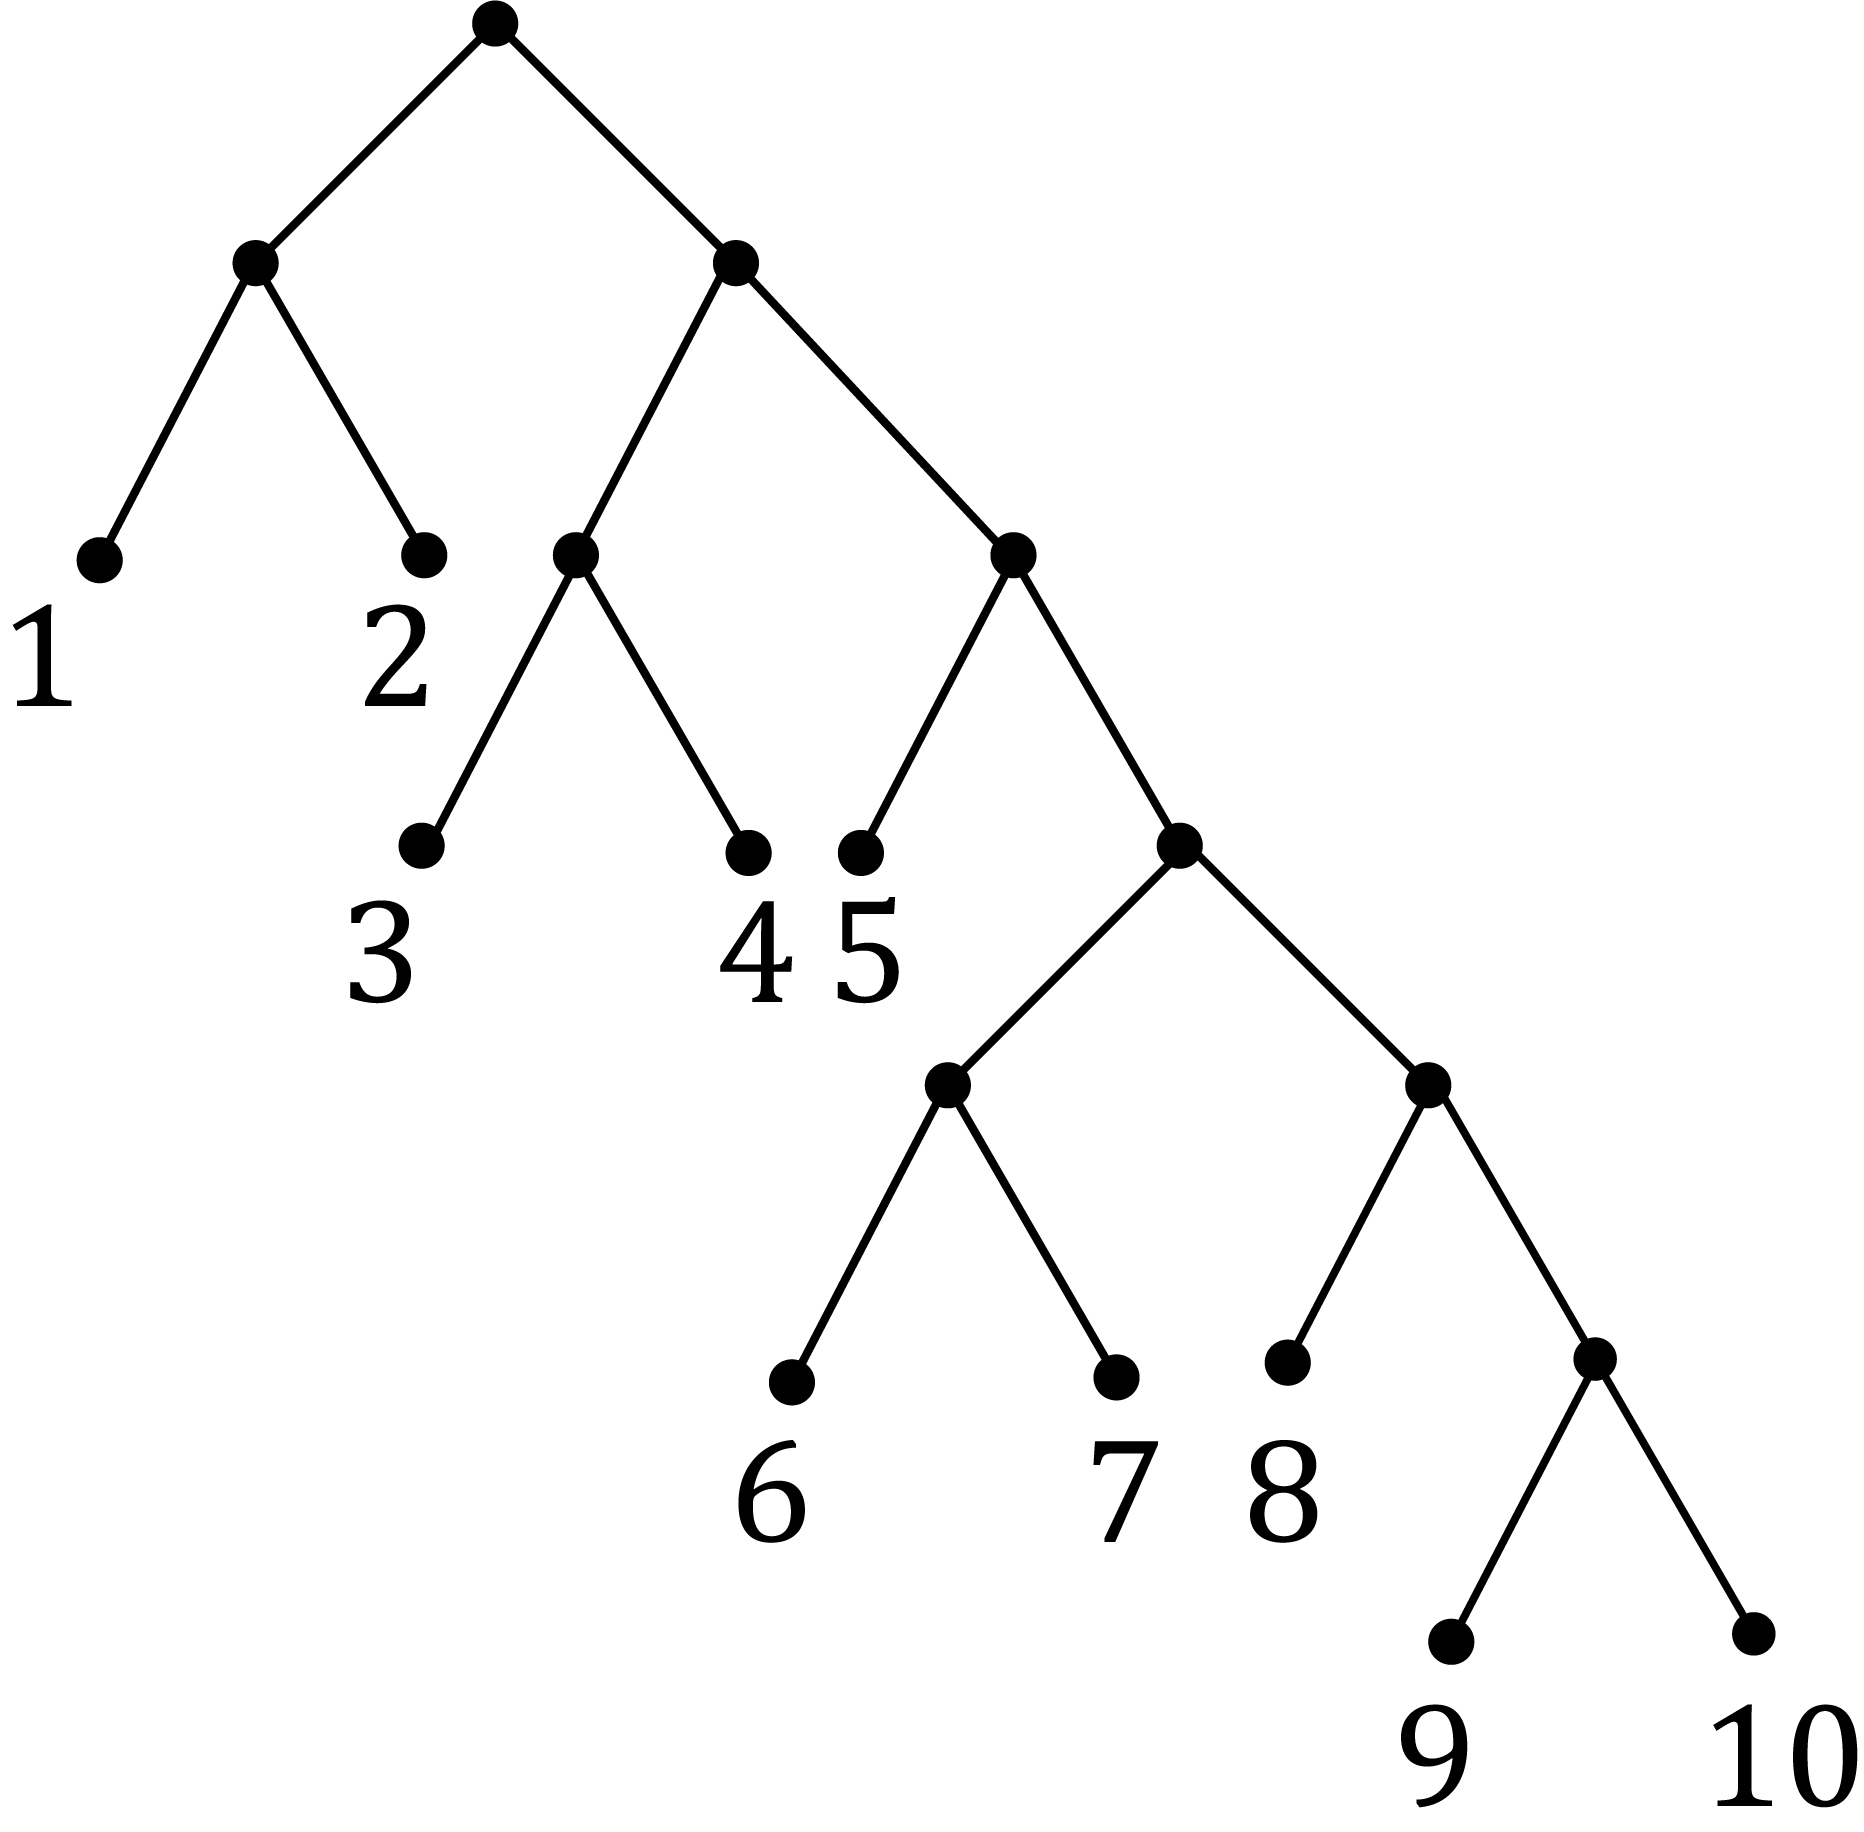
\includegraphics[width=15cm]{pics/18_1.png}
        \centering
    \end{figure}
  \end{proof}
\end{document}
